%\iffalse
\let\negmedspace\undefined
\let\negthickspace\undefined
\documentclass[journal,12pt,twocolumn]{IEEEtran}
\usepackage{cite}
\usepackage{amsmath,amssymb,amsfonts,amsthm}
\usepackage{algorithmic}
\usepackage{graphicx}
\usepackage{textcomp}
\usepackage{xcolor}
\usepackage{txfonts}
\usepackage{listings}
\usepackage{enumitem}
\usepackage{mathtools}
\usepackage{gensymb}
\usepackage{comment}
\usepackage[breaklinks=true]{hyperref}
\usepackage{tkz-euclide} 
\usepackage{listings}
\usepackage{gvv}                                        
\def\inputGnumericTable{}                                 
\usepackage[latin1]{inputenc}                                
\usepackage{color}                                            
\usepackage{array}                                            
\usepackage{longtable}                                       
\usepackage{calc}                                             
\usepackage{multirow}                                         
\usepackage{hhline}                                           
\usepackage{ifthen}                                           
\usepackage{lscape}
\usepackage{circuitikz}
\newtheorem{theorem}{Theorem}[section]
\newtheorem{problem}{Problem}
\newtheorem{proposition}{Proposition}[section]
\newtheorem{lemma}{Lemma}[section]
\newtheorem{corollary}[theorem]{Corollary}
\newtheorem{example}{Example}[section]
\newtheorem{definition}[problem]{Definition}
\newcommand{\BEQA}{\begin{eqnarray}}
\newcommand{\EEQA}{\end{eqnarray}}
\newcommand{\define}{\stackrel{\triangle}{=}}
\theoremstyle{remark}
\newtheorem{rem}{Remark}
\begin{document}
\parindent 0px

\bibliographystyle{IEEEtran}
\vspace{3cm}

\title{Assignment\\[1ex]GATE-EC-39}
\author{EE23BTECH11034 - Prabhat Kukunuri$^{}$% <-this % stops a space
}
\maketitle
\newpage
\bigskip

\renewcommand{\thefigure}{\theenumi}
\renewcommand{\thetable}{\theenumi}
\section{Question}
Consider a polar non-return to zero \brak{NRZ} waveform, using $+2V$ and $-2V$ for representing binary '1' and '0' respectively, is transmitted in the presence of additive zero-mean white Gaussian noise with variance 0.4 $V^2$. If the a $priori$ probability of transmission of a binary '1' is 0.4, the optimum threshold voltage for a maximum a $posteriori$\brak{MAP}receiver (rounded off to two decimal places) is \rule{1.5cm}{0.15mm}V.

\solution
\begin{table}[h]
    \centering
    \begin{tabular}{|p{1cm}|p{3.80cm}|p{2.70cm}|}
    \hline
    Symbol&Value&Description\\ \hline
    $$v_{th}$$&$$\frac{a_1+a_2}{2}+\frac{\sigma_{n}^{2}}{a_1-a_2}ln\brak{\frac{P\brak{0}}{P\brak{1}}}$$&optimum threshold value\\\hline
    $$P\brak{0}$$&$$0.6$$&Probability of error when 0 is transmitted\\\hline
    $$P\brak{1}$$&$$0.4$$&Probability of error when 1 is transmitted\\\hline
    $$\sigma_{n}^{2}$$&$$0.4V^2$$&Variance of the noise\\\hline
    $$a_1$$&$$E\sbrak{X+N}$$&voltage of transmission for binary 1\\\hline
    $$a_2$$&$$E\sbrak{X+N}$$&voltage of transmission for binary 0\\\hline
    \end{tabular}
    \caption{Variable description}
    \label{tab:GATE.2022.EC.53.1}
\end{table}\\
\begin{align}
    &a_1=E\sbrak{X+N}\\
    &a_1=E\sbrak{X}+E\sbrak{N}\\
    &\text{Given mean noise is zero}\brak{E\sbrak{N}=0}\\
    &a_1=E\sbrak{2}\\
    &a_1=2
\end{align}
Similarly,
\begin{align}
    &a_2=E\sbrak{X+N}\\
    &a_2=E\sbrak{-2}+E\sbrak{N}\\
    &a_2=-2
\end{align}
Optimum threshold voltage is,
\begin{align}
    &v_{th}=\frac{2-2}{2}+\frac{0.4}{2-\brak{-2}}ln\brak{\frac{0.6}{0.4}}\\
    &v_{th}=0.04V
\end{align}
\begin{figure}[ht]
    \centering
    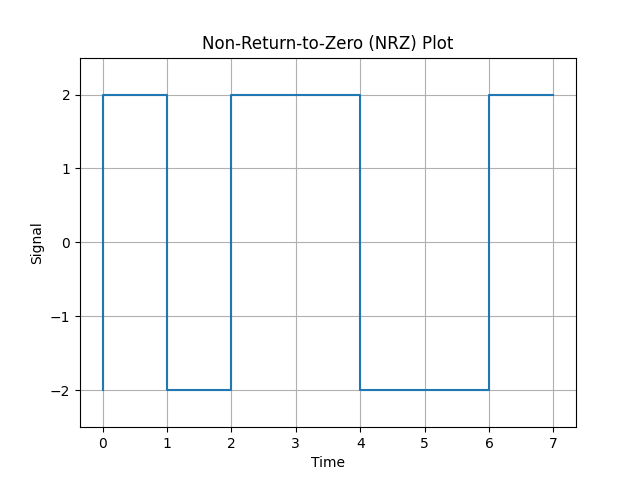
\includegraphics[width=\columnwidth]{figs/Figure_1.png}
    \caption{Plot of x(n) $vs$ n}
    \label{fig:GATE.2022.EC.53.2}
\end{figure}
\end{document}